\documentclass[tikz,border=12pt]{standalone}
\usepackage[T1]{fontenc}
\usepackage{tgheros}
\usepackage{sfmath}
\usepackage{amsmath}
\usepackage{fontawesome5}
\usepackage{tikz}
\usetikzlibrary{arrows.meta,positioning,shapes.geometric,fit,backgrounds,calc}
\usepackage{xcolor}

\renewcommand{\familydefault}{\sfdefault}

% Harvard Crimson & ETH Zurich Academic Semantic Palette
\definecolor{harvardcrimson}{HTML}{A51C30}
\definecolor{ethdarkblue}{HTML}{1F407A}
\definecolor{ethblue}{HTML}{215CAF}
\definecolor{ethpetrol}{HTML}{007A87}
\definecolor{ethbronze}{HTML}{B87333}
\definecolor{ethpurple}{HTML}{5B4B8A}
\definecolor{ethslate}{HTML}{475569}
\definecolor{cardbg}{HTML}{F8FAFC}
\definecolor{cardborder}{HTML}{CBD5E1}
\definecolor{safeTeal}{HTML}{10B981}

\begin{document}
\begin{tikzpicture}[
  font=\sffamily,
  >=Stealth,
  stagebox/.style={
    draw=cardborder,
    fill=cardbg,
    rounded corners=4pt,
    line width=0.8pt,
    text width=1.12in,
    minimum height=1.65in,
    inner sep=6pt,
    align=center,
    anchor=north
  }
]

  % Top Title Banner
  \node[draw=ethdarkblue, fill=ethdarkblue!5, rounded corners=5pt, line width=1pt, text width=8.70in, inner sep=7pt, align=center] (title) at (4.35in, 0) {
    {\normalsize\bfseries\color{ethdarkblue}\faIcon{clock}\;\; THE 7-STAGE SENSE-TO-ACTUATION LATENCY WATERFALL}\\[2pt]
    {\scriptsize\color{ethslate}Where Does the Time Go? Deconstructing the Physical, Memory, Neural, and Silicon Bottlenecks}
  };

  % 7 Stages Across the Pipeline
  \node[stagebox, draw=ethblue!70] (st1) at (0, -0.65in) {
    {\scriptsize\bfseries\color{ethblue}\faIcon{satellite-dish}\; STAGE 1}\\[3pt]
    {\scriptsize\bfseries Transduce}\\[4pt]
    {\tiny\color{ethslate}Photodiode Well Exposure \& IMU Deflection}\\[6pt]
    \rule{0.9\linewidth}{0.3pt}\\[4pt]
    {\scriptsize\textbf{\color{safeTeal}$P_{50}$: $8\text{ ms}$}}\\[1pt]
    {\scriptsize\textbf{\color{harvardcrimson}$P_{99}$: $15\text{ ms}$}}
  };

  \node[stagebox, draw=ethpetrol!70] (st2) at (1.26in, -0.65in) {
    {\scriptsize\bfseries\color{ethpetrol}\faIcon{microchip}\; STAGE 2}\\[3pt]
    {\scriptsize\bfseries DMA Ingest}\\[4pt]
    {\tiny\color{ethslate}MIPI CSI-2 Bus Transfer into Shared DRAM}\\[6pt]
    \rule{0.9\linewidth}{0.3pt}\\[4pt]
    {\scriptsize\textbf{\color{safeTeal}$P_{50}$: $3\text{ ms}$}}\\[1pt]
    {\scriptsize\textbf{\color{harvardcrimson}$P_{99}$: $8\text{ ms}$}}
  };

  \node[stagebox, draw=ethblue!80] (st3) at (2.52in, -0.65in) {
    {\scriptsize\bfseries\color{ethblue}\faIcon{eye}\; STAGE 3}\\[3pt]
    {\scriptsize\bfseries Perception}\\[4pt]
    {\tiny\color{ethslate}ViT Encoders \& DINOv2\\[1pt]3D Spatial Tokens}\\[6pt]
    \rule{0.9\linewidth}{0.3pt}\\[4pt]
    {\scriptsize\textbf{\color{safeTeal}$P_{50}$: $12\text{ ms}$}}\\[1pt]
    {\scriptsize\textbf{\color{harvardcrimson}$P_{99}$: $25\text{ ms}$}}
  };

  \node[stagebox, draw=ethbronze!90] (st4) at (3.78in, -0.65in) {
    {\scriptsize\bfseries\color{ethbronze}\faIcon{brain}\; STAGE 4}\\[3pt]
    {\scriptsize\bfseries Policy VLA}\\[4pt]
    {\tiny\color{ethslate}Diffusion ACT / VLA\\[1pt]Action Chunk Pass}\\[6pt]
    \rule{0.9\linewidth}{0.3pt}\\[4pt]
    {\scriptsize\textbf{\color{safeTeal}$P_{50}$: $22\text{ ms}$}}\\[1pt]
    {\scriptsize\textbf{\color{harvardcrimson}$P_{99}$: $60\text{ ms}$}}
  };

  \node[stagebox, draw=ethpurple!80] (st5) at (5.04in, -0.65in) {
    {\scriptsize\bfseries\color{ethpurple}\faIcon{network-wired}\; STAGE 5}\\[3pt]
    {\scriptsize\bfseries Inter-IPC}\\[4pt]
    {\tiny\color{ethslate}Shared SRAM Mailbox\\[1pt]RPMSG MPU-to-MCU}\\[6pt]
    \rule{0.9\linewidth}{0.3pt}\\[4pt]
    {\scriptsize\textbf{\color{safeTeal}$P_{50}$: $0.8\text{ ms}$}}\\[1pt]
    {\scriptsize\textbf{\color{harvardcrimson}$P_{99}$: $2.0\text{ ms}$}}
  };

  \node[stagebox, draw=ethpetrol!90] (st6) at (6.30in, -0.65in) {
    {\scriptsize\bfseries\color{ethpetrol}\faIcon{shield-alt}\; STAGE 6}\\[3pt]
    {\scriptsize\bfseries Enforce}\\[4pt]
    {\tiny\color{ethslate}1 kHz CBF Filter \&\\[1pt]Stopping Distance}\\[6pt]
    \rule{0.9\linewidth}{0.3pt}\\[4pt]
    {\scriptsize\textbf{\color{safeTeal}$P_{50}$: $0.4\text{ ms}$}}\\[1pt]
    {\scriptsize\textbf{\color{harvardcrimson}$P_{99}$: $1.0\text{ ms}$}}
  };

  \node[stagebox, draw=harvardcrimson!80] (st7) at (7.56in, -0.65in) {
    {\scriptsize\bfseries\color{harvardcrimson}\faIcon{cogs}\; STAGE 7}\\[3pt]
    {\scriptsize\bfseries Actuator}\\[4pt]
    {\tiny\color{ethslate}Motor Stator $L/R$ Coil\\[1pt]Current Rise to Torque}\\[6pt]
    \rule{0.9\linewidth}{0.3pt}\\[4pt]
    {\scriptsize\textbf{\color{safeTeal}$P_{50}$: $6\text{ ms}$}}\\[1pt]
    {\scriptsize\textbf{\color{harvardcrimson}$P_{99}$: $15\text{ ms}$}}
  };

  % Timeline Comparisons at Bottom with Generous Vertical Clearance
  % NOMINAL P50 BAR
  \node[anchor=west, font=\sffamily\bfseries\scriptsize, text=safeTeal] at (0, -2.90in) {\faIcon{check-circle}\; Nominal Path ($P_{50} = 52.2\text{ ms}$):};
  \draw[fill=safeTeal!20, draw=safeTeal, line width=1pt, rounded corners=3pt] (2.40in, -3.00in) rectangle ++(3.13in, 0.22in);
  \node[font=\sffamily\bfseries\tiny, text=safeTeal!90] at (3.96in, -2.89in) {Safe Closed-Loop Margin ($52.2\text{ ms} \ll \tau_{\text{world}}$)};

  % TAIL P99 BAR
  \node[anchor=west, font=\sffamily\bfseries\scriptsize, text=harvardcrimson] at (0, -3.25in) {\faIcon{exclamation-triangle}\; Tail Path ($P_{99} = 126.0\text{ ms}$):};
  \draw[fill=harvardcrimson!20, draw=harvardcrimson, line width=1pt, rounded corners=3pt] (2.40in, -3.35in) rectangle ++(6.30in, 0.22in);
  \node[font=\sffamily\bfseries\tiny, text=harvardcrimson] at (5.55in, -3.24in) {CRITICAL TIMING VIOLATION ($126.0\text{ ms} > \tau_{\text{world}}$)};

  % World Deadline Vertical Marker (Safely Positioned Below Stage 7)
  \draw[dashed, line width=1.3pt, draw=harvardcrimson!90] (7.40in, -2.68in) -- (7.40in, -3.50in);
  \node[font=\sffamily\bfseries\tiny, fill=white, draw=harvardcrimson, rounded corners=2pt, inner sep=2pt, text=harvardcrimson] at (7.40in, -2.60in) {World Deadline $\tau_{\text{world}} = 100\text{ ms}$};

\end{tikzpicture}
\end{document}
